



\tikzset{every picture/.style={line width=0.75pt}} %set default line width to 0.75pt        

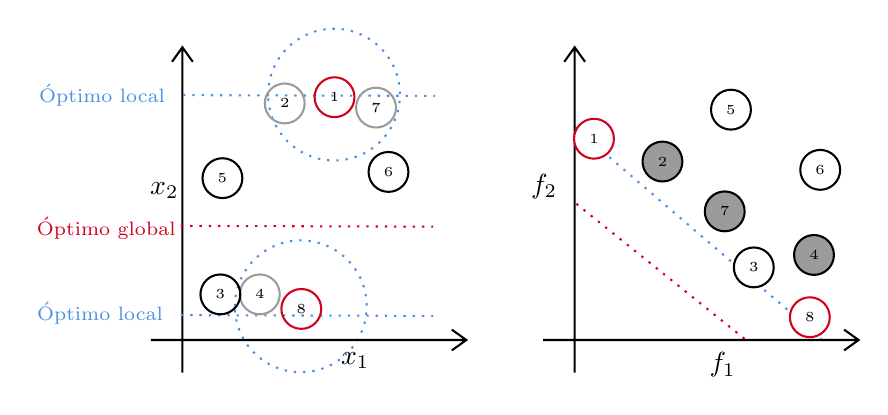
\begin{tikzpicture}[x=0.75pt,y=0.75pt,yscale=-1,xscale=1]
%uncomment if require: \path (0,300); %set diagram left start at 0, and has height of 300

%Shape: Circle [id:dp5136866411017809] 
\draw  [color={rgb, 255:red, 74; green, 144; blue, 226 }  ,draw opacity=1 ][dash pattern={on 0.84pt off 2.51pt}] (133,181.75) .. controls (133,164.21) and (147.21,150) .. (164.75,150) .. controls (182.29,150) and (196.5,164.21) .. (196.5,181.75) .. controls (196.5,199.29) and (182.29,213.5) .. (164.75,213.5) .. controls (147.21,213.5) and (133,199.29) .. (133,181.75) -- cycle ;
%Shape: Axis 2D [id:dp3645341276574614] 
\draw  (92.5,197.98) -- (244.5,197.98)(107.7,56.94) -- (107.7,213.65) (237.5,192.98) -- (244.5,197.98) -- (237.5,202.98) (102.7,63.94) -- (107.7,56.94) -- (112.7,63.94)  ;
%Straight Lines [id:da5028238368202924] 
\draw [color={rgb, 255:red, 74; green, 144; blue, 226 }  ,draw opacity=1 ] [dash pattern={on 0.84pt off 2.51pt}]  (296.5,95.37) -- (415.5,197.37) ;


%Straight Lines [id:da41718558536419126] 
\draw [color={rgb, 255:red, 208; green, 2; blue, 27 }  ,draw opacity=1 ] [dash pattern={on 0.84pt off 2.51pt}]  (297.5,132.37) -- (378.5,197.37) ;


%Straight Lines [id:da19270549692989558] 
\draw [color={rgb, 255:red, 74; green, 144; blue, 226 }  ,draw opacity=1 ] [dash pattern={on 0.84pt off 2.51pt}]  (108,80) -- (229.5,80.37) ;


%Straight Lines [id:da6200442991423092] 
\draw [color={rgb, 255:red, 208; green, 2; blue, 27 }  ,draw opacity=1 ] [dash pattern={on 0.84pt off 2.51pt}]  (107,143) -- (228.5,143.37) ;


%Shape: Axis 2D [id:dp245732011351129] 
\draw  (281.5,197.98) -- (433.5,197.98)(296.7,56.94) -- (296.7,213.65) (426.5,192.98) -- (433.5,197.98) -- (426.5,202.98) (291.7,63.94) -- (296.7,56.94) -- (301.7,63.94)  ;
%Straight Lines [id:da28170380219279356] 
\draw [color={rgb, 255:red, 74; green, 144; blue, 226 }  ,draw opacity=1 ] [dash pattern={on 0.84pt off 2.51pt}]  (107,186) -- (228.5,186.37) ;


%Shape: Circle [id:dp048880164221430045] 
\draw  [color={rgb, 255:red, 74; green, 144; blue, 226 }  ,draw opacity=1 ][dash pattern={on 0.84pt off 2.51pt}] (149,79.75) .. controls (149,62.21) and (163.21,48) .. (180.75,48) .. controls (198.29,48) and (212.5,62.21) .. (212.5,79.75) .. controls (212.5,97.29) and (198.29,111.5) .. (180.75,111.5) .. controls (163.21,111.5) and (149,97.29) .. (149,79.75) -- cycle ;

% Text Node
\draw  [color={rgb, 255:red, 208; green, 2; blue, 27 }  ,draw opacity=1 ]  (181, 81) circle [x radius= 9.6, y radius= 9.6]   ;
\draw (181,81) node  [font=\tiny] [align=left] {1};
% Text Node
\draw  [color={rgb, 255:red, 0; green, 0; blue, 0 }  ,draw opacity=1 ]  (127, 120) circle [x radius= 9.6, y radius= 9.6]   ;
\draw (127,120) node  [font=\tiny] [align=left] {5};
% Text Node
\draw  [color={rgb, 255:red, 155; green, 155; blue, 155 }  ,draw opacity=1 ]  (157, 84) circle [x radius= 9.6, y radius= 9.6]   ;
\draw (157,84) node  [font=\tiny] [align=left] {2};
% Text Node
\draw    (207, 117) circle [x radius= 9.6, y radius= 9.6]   ;
\draw (207,117) node  [font=\tiny] [align=left] {6};
% Text Node
\draw  [color={rgb, 255:red, 155; green, 155; blue, 155 }  ,draw opacity=1 ]  (201, 86) circle [x radius= 9.6, y radius= 9.6]   ;
\draw (201,86) node  [font=\tiny] [align=left] {7};
% Text Node
\draw  [color={rgb, 255:red, 155; green, 155; blue, 155 }  ,draw opacity=1 ]  (145, 176) circle [x radius= 9.6, y radius= 9.6]   ;
\draw (145,176) node  [font=\tiny] [align=left] {4};
% Text Node
\draw  [color={rgb, 255:red, 208; green, 2; blue, 27 }  ,draw opacity=1 ]  (165, 183) circle [x radius= 9.6, y radius= 9.6]   ;
\draw (165,183) node  [font=\tiny] [align=left] {8};
% Text Node
\draw    (126, 176) circle [x radius= 9.6, y radius= 9.6]   ;
\draw (126,176) node  [font=\tiny] [align=left] {3};
% Text Node
\draw  [color={rgb, 255:red, 208; green, 2; blue, 27 }  ,draw opacity=1 ][fill={rgb, 255:red, 255; green, 255; blue, 255 }  ,fill opacity=1 ]  (306, 101) circle [x radius= 9.6, y radius= 9.6]   ;
\draw (306,101) node  [font=\tiny] [align=left] {1};
% Text Node
\draw  [color={rgb, 255:red, 0; green, 0; blue, 0 }  ,draw opacity=1 ][fill={rgb, 255:red, 255; green, 255; blue, 255 }  ,fill opacity=1 ]  (372, 87) circle [x radius= 9.6, y radius= 9.6]   ;
\draw (372,87) node  [font=\tiny] [align=left] {5};
% Text Node
\draw  [color={rgb, 255:red, 0; green, 0; blue, 0 }  ,draw opacity=1 ][fill={rgb, 255:red, 155; green, 155; blue, 155 }  ,fill opacity=1 ]  (339, 112) circle [x radius= 9.6, y radius= 9.6]   ;
\draw (339,112) node  [font=\tiny] [align=left] {2};
% Text Node
\draw  [fill={rgb, 255:red, 255; green, 255; blue, 255 }  ,fill opacity=1 ]  (415, 116) circle [x radius= 9.6, y radius= 9.6]   ;
\draw (415,116) node  [font=\tiny] [align=left] {6};
% Text Node
\draw  [color={rgb, 255:red, 0; green, 0; blue, 0 }  ,draw opacity=1 ][fill={rgb, 255:red, 155; green, 155; blue, 155 }  ,fill opacity=1 ]  (369, 136) circle [x radius= 9.6, y radius= 9.6]   ;
\draw (369,136) node  [font=\tiny] [align=left] {7};
% Text Node
\draw  [fill={rgb, 255:red, 155; green, 155; blue, 155 }  ,fill opacity=1 ]  (412, 157) circle [x radius= 9.6, y radius= 9.6]   ;
\draw (412,157) node  [font=\tiny] [align=left] {4};
% Text Node
\draw  [color={rgb, 255:red, 208; green, 2; blue, 27 }  ,draw opacity=1 ][fill={rgb, 255:red, 255; green, 255; blue, 255 }  ,fill opacity=1 ]  (410, 187) circle [x radius= 9.6, y radius= 9.6]   ;
\draw (410,187) node  [font=\tiny] [align=left] {8};
% Text Node
\draw  [fill={rgb, 255:red, 255; green, 255; blue, 255 }  ,fill opacity=1 ]  (383, 163) circle [x radius= 9.6, y radius= 9.6]   ;
\draw (383,163) node  [font=\tiny] [align=left] {3};
% Text Node
\draw (191,208) node    {$x_{1}$};
% Text Node
\draw (99,126) node    {$x_{2}$};
% Text Node
\draw (368,210) node    {$f_{1}$};
% Text Node
\draw (282,124) node    {$f_{2}$};
% Text Node
\draw (69,80) node  [font=\scriptsize,color={rgb, 255:red, 74; green, 144; blue, 226 }  ,opacity=1 ] [align=left] {Óptimo local};
% Text Node
\draw (68,185) node  [font=\scriptsize,color={rgb, 255:red, 74; green, 144; blue, 226 }  ,opacity=1 ] [align=left] {Óptimo local};
% Text Node
\draw (71,144) node  [font=\scriptsize,color={rgb, 255:red, 208; green, 2; blue, 27 }  ,opacity=1 ] [align=left] {Óptimo global};


\end{tikzpicture}
